\documentclass[]{report}
\usepackage{graphicx}
\usepackage{float}
\usepackage{amsmath}
\usepackage{amsfonts}
\usepackage{wasysym}
\usepackage{listings}
\usepackage{xcolor}
\lstset{
	basicstyle=\ttfamily,
	columns=fullflexible,
	frame=L,
	showstringspaces=false, 
	commentstyle=\color{green},
	breaklines=true,
	postbreak=\mbox{\textcolor{red}{$\hookrightarrow$}\space},
}
\pagenumbering{Roman}
% Title Page
\title{MCEN - 3047}
\author{Jack Goldrick}


\begin{document}
	\maketitle
	
	\section{Problem 1}
	
	\subsection{Part A}
	
\begin{figure}[h]
	\centering
	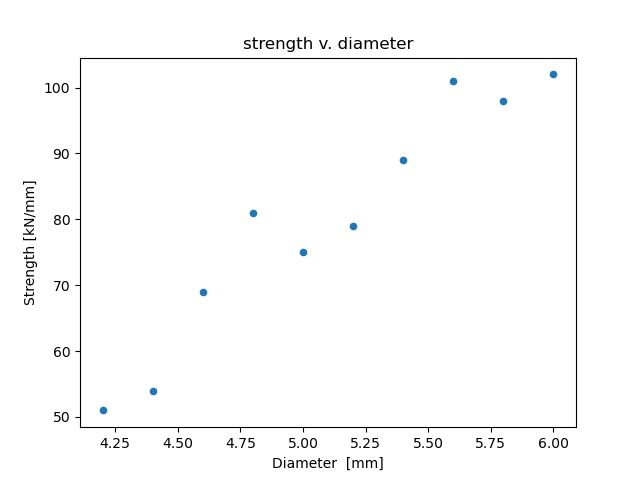
\includegraphics[width=0.7\linewidth]{pics/1a}
	\label{fig:1a}
\end{figure}


\begin{itemize}
	\item A linear Model may work here. However, the plot has a general linear trend, I believe the $R^2$ should be at least 80
\end{itemize}
	
	\subsection{Part C}
	
	\begin{figure}[h]
		\centering
		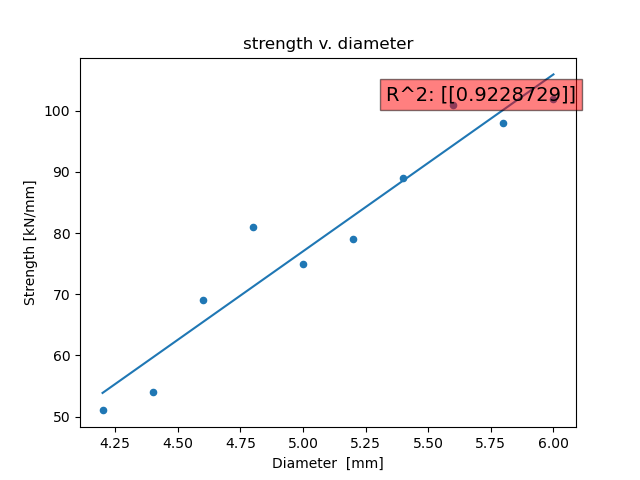
\includegraphics[width=0.7\linewidth]{pics/1bc}
		\label{fig:1c}
	\end{figure}
	
	
	\subsection{Part E}
	
	\begin{figure}[h]
		\centering
		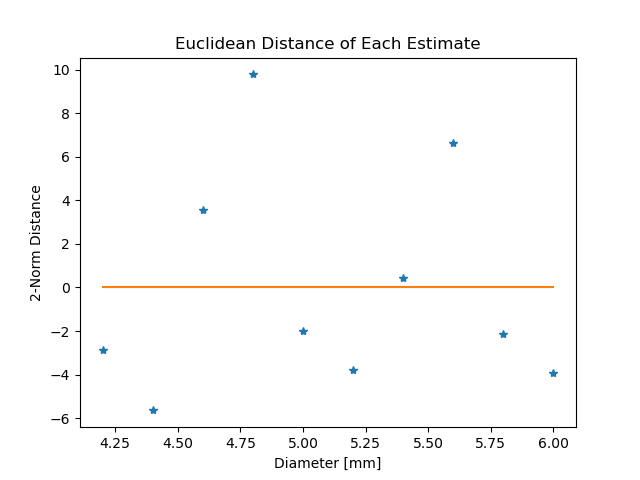
\includegraphics[width=0.7\linewidth]{pics/1e}
		\label{fig:1e}
	\end{figure}
	
	\subsection{Part F}
	
	\begin{itemize}
		\item  8.68175868988037 kN
	\end{itemize}
	
	\subsection{Part G}
	
	\begin{itemize}
		\item  91.62211608886719 kN
	\end{itemize}
	
	\subsection{Part H}
	
		\begin{itemize}
		\item While we can calculate a value.  Given the lack of knowledge, we cannot use this local behavior to predict global behavior. Thus it is not advised as a valid methodology.
	\end{itemize}
	\section{CODE}
	
	\subsection{Part I}
	
	\begin{itemize}
		\item 5.6218mm
	\end{itemize}
	
	\newpage
	
	\section{Problem 2}
	
	\subsection{Part A}
	
		\begin{figure}[h]
		\centering
		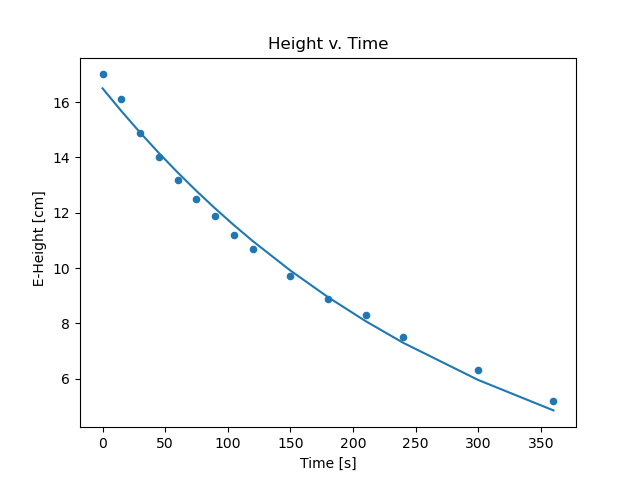
\includegraphics[width=0.7\linewidth]{pics/2}
		\label{fig:2}
	\end{figure}
	
	\subsection{Part B}


	\begin{itemize}
		\item 294.4462890625
	\end{itemize}
	
	
	\newpage
	
	\section{Problem 3}
	
	
			\begin{figure}[h]
		\centering
		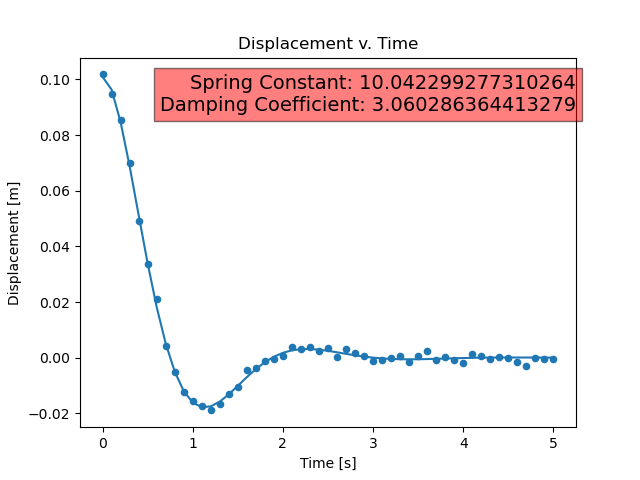
\includegraphics[width=0.7\linewidth]{pics/3}
		\label{fig:3}
	\end{figure}
	
	
	\begin{lstlisting}[language=Python]
		
		import torch as tc
		import numpy as np
		import matplotlib.pyplot as plt
		import pandas as pd
		from scipy.optimize import curve_fit
		
		
		def get_df(file_path):
		df = pd.read_csv(file_path)
		return df
		
		def quick_scatter(df, curve=None, title=None, text=None):
		graph = df.plot.scatter(x=0, y=1, title=title)
		if curve is not None:
		graph.plot(curve[0], curve[1])
		if text is not None:
		
		plt.text(1, .9, s=text, fontsize = 14, ha='right', va='center', transform=plt.gca().transAxes,
		bbox = dict(facecolor = 'red', alpha = 0.5))
		plt.show()
		
		def resid_scatter(resids, input):
		plt.plot(input, resids, '*')
		plt.plot(input, np.zeros(len(input)))
		plt.title("Euclidean Distance of Each Estimate")
		plt.ylabel("2-Norm Distance")
		plt.xlabel("Diameter [mm]")
		plt.show()
		
		# Create a tensor from a csv file
		def tensorize_df(df):
		# print(data.head())
		# Convert the data to a numpy array
		data = df.to_numpy()
		x1 = data[:, 1]
		x0 = data[:, 0]
		
		return tc.tensor(x1, dtype=tc.float), tc.tensor(x0, dtype=tc.float)
		
		
		# Exponential decay function
		def non_linear_least_squares(input, output, h_0=15, tau=100, tol = 1e-7):
		
		error = 100
		error_seq = 100
		
		resid = output - h_0 * tc.exp(- input / tau)
		
		while error_seq > tol:
		
		
		dh_0 = tc.exp(-input / tau)
		dtau = h_0 * input * tc.exp(-input / tau) * tau**(-2)
		
		J = tc.stack([dh_0, dtau], dim=1)
		
		J_dual = J.mT
		
		del_coeff = tc.inverse(J_dual @ J) @ J_dual @ resid
		# print(del_coeff)
		
		h_0 = h_0 + del_coeff[0]
		tau = tau + del_coeff[1]
		
		resid = output - h_0 * tc.exp(- input / tau)
		# import pdb; pdb.set_trace()
		error = tc.sqrt(resid.unsqueeze(0) @ resid)
		
		error_seq = tc.abs(del_coeff[0] / h_0) + tc.abs( del_coeff[1] / tau) 
		
		
		
		
		
		final_coeff = [h_0, tau]
		output = h_0 * tc.exp(- input / tau)
		
		return final_coeff, output, error, error_seq
		
		def calc_error(tensor, output,  coeff, resid=False):
		
		# output = output.to(tc.float)
		error_vect = output - (tensor @ coeff)
		
		
		if resid:
		r_squared = error_vect @ error_vect
		r = tc.sqrt(r_squared)
		return r, r_squared
		
		
		dim = len(output)
		output = output.unsqueeze(0)
		tensor_dual = tensor.mT
		
		t_gram = tensor_dual @ tensor
		
		tensor_gram_inv = tc.inverse(t_gram)
		
		P = tensor @ tensor_gram_inv @ tensor_dual
		
		M = tc.eye(dim, dtype=tc.float) - P
		
		L = tc.eye(dim, dtype=tc.float) - tc.ones(dim, dim, dtype=tc.float) / dim
		
		# import pdb; pdb.set_trace()
		rss = output @ M @ output.mT
		# import pdb; pdb.set_trace()
		tss = output @ L @ output.mT
		
		r_squared = 1 - (rss / tss)
		
		return r_squared
		
		# r_squared = 1 - (tc.norm(error_vect) / tc.norm(output))
		
		
		def least_squares(input, output, order=1, resid=False, time_span=None):
		
		""" 
		-- The alg represents the equation Ax = b
		where A is the input matrix, x is the unknown vector
		of linear coefficients and b is the output vector.
		-- We are attempting to minimize the max error between
		points in a metric space represented by the Feature 
		Space.
		-- The function returns the vector x.
		"""
		
		
		# Create the input matrix
		A = tc.tensor([[i**j for j in range(order+1)] for i in input], dtype=tc.float)
		
		A_dual = A.mT
		
		A_gram = A_dual @ A
		
		A_gram_inv = tc.inverse(A_gram)
		
		coeff = A_gram_inv @ A_dual @ output
		
		# print(coeff)
		
		if time_span is None:
		out_est = A @ coeff
		else:
		time = tc.linspace(start=time_span[0],steps=time_span[1] , end=time_span[2])
		
		if resid:
		return coeff.numpy(), out_est.numpy(), calc_error(tensor=A, output=output, coeff=coeff, resid=True)
		
		return coeff.numpy(), out_est.numpy(), calc_error(tensor=A, output=output, coeff=coeff)
		
		
		def model(t, A, phi, b, omega_d):
		
		
		return (A * np.exp(-b *.5 * t) * np.cos(omega_d * t + phi))
		
		
		
		def estimate_spring(x, t, initial_guess=None):
		if initial_guess is None:
		initial_guess = [1, 1, 1, 1]
		# import pdb; pdb.set_trace()
		params, covariance = curve_fit(model, xdata=t.numpy(), ydata=x.numpy(), p0=initial_guess)
		
		# Extract estimated parameters
		A_est, phi_est, beta_est, omega_est = params
		# print(params)
		
		return A_est, phi_est, beta_est, omega_est
		
		
		def problem_1(order=1):
		df = get_df("../data/p1.csv")
		quick_scatter(df, title="strength v. diameter")
		stre, dia = tensorize_df(df)
		coeff, output, error = least_squares(output=stre, input=dia, order=order)
		notes = f"R^2: {error.numpy()}"
		quick_scatter(df, title="strength v. diameter", curve=[dia, output], text=notes)
		time = tc.linspace(start=5, steps=100, end=6)
		
		A = tc.tensor([[i**j for j in range(order+1)] for i in time], dtype=tc.float)
		est_out = A @ coeff
		resid = stre.numpy() - output
		resid_scatter(input=dia.numpy(), resids=resid)
		# print(time[50])
		print(f"Strength change for dx = .3mm: {coeff[1] * .3 }")
		print(f"Strength at 5.5mm: {est_out[50]}")
		
		
		
		
		
		
		def problem_2():
		df = get_df("../data/beer.csv")
		
		height, time = tensorize_df(df)
		final_coeff, output, error, _ = non_linear_least_squares(input=time, output=height)
		
		
		quick_scatter(df, curve=[time, output], title="Height v. Time")
		
		print(f"Time constant: {final_coeff[1].numpy()}")
		
		
		def problem_3():
		df = get_df("../data/p3.csv")
		
		x, t = tensorize_df(df)
		
		# print(t)
		# import pdb; pdb.set_trace()
		
		_, _, b_est, omega_d_est = estimate_spring(x=x, t=t)
		
		k_est = omega_d_est**2 + .25 * b_est**2
		notes = f"Spring Constant: {k_est}\nDamping Coefficient: {b_est}"
		quick_scatter(df, title="Displacement v. Time", curve=[t, model(t, *estimate_spring(x, t))], text=notes)
		
		
		
		
		def main():
		problem_1()
		problem_2()
		problem_3()
		main()
		
		
		
	\end{lstlisting}
	
\end{document}          




